% ============================================================
% ICLR 2026 Poster: Understanding the Mechanisms of
% Fast Hyperparameter Transfer (Ghosh, Wu, Bietti)
%
% Landscape 190 x 90 cm. Compile with tectonic (or Overleaf).
% ============================================================

\documentclass{beamer}

\usepackage[orientation=landscape,size=custom,width=190,height=90,scale=1.25]{beamerposter}

\usetheme{metropolis}

% Suppress any beamer/metropolis cruft that would show up on a poster
\setbeamertemplate{navigation symbols}{}
\setbeamertemplate{headline}{}
\setbeamertemplate{footline}{}
\setbeamertemplate{frametitle}{}
\setbeamersize{text margin left=0.8em, text margin right=0.8em}

% Math + graphics
\usepackage{amsmath, amssymb, amsfonts, bm}
\usepackage{graphicx}
\usepackage{tikz}
\usetikzlibrary{arrows.meta, calc}

% Colors + highlight-box macros (\redbox, \bluebox, \tealbox, \orangebox)
% ======================================================================
% Preamble for the ICLR 2026 poster.
% Colors copied from HP_Transfer__slides_/main.tex:142-185.
% Highlight-box macros copied from HP_Transfer__slides_/main.tex:249-283.
% ======================================================================

\usepackage{xcolor}

% matplotlib defaults
\definecolor{C0}{HTML}{1f77b4}
\definecolor{C1}{HTML}{ff7f0e}

% Vector colors
\definecolor{tangocolorvectorred}{HTML}{E40086}
\definecolor{tangocolorvectorblue}{HTML}{014171}
\definecolor{tangocolorvectorpurple}{HTML}{861e80}
\definecolor{tangocolorvectorlightblue}{HTML}{4C6379}
\definecolor{tangocolorvectordarkblue}{HTML}{07223E}

% NYU & Flatiron
\definecolor{FlatironOrange2}{HTML}{f5862d}

% tango plum
\definecolor{tangocolordarkplum}{HTML}{5C3566}
\definecolor{tangocolormediumplum}{HTML}{75507B}
\definecolor{tangocolorlightplum}{HTML}{AD7FA8}

% scarlet red
\definecolor{tangocolordarkscarletred}{HTML}{A40000}
\definecolor{tangocolormediumscarletred}{HTML}{CC0000}
\definecolor{tangocolorlightscarletred}{HTML}{EF2929}

% aluminium
\definecolor{tangocolordarkaluminium}{HTML}{BABDB6}
\definecolor{tangocolormediumaluminium}{HTML}{D3D3D3}
\definecolor{tangocolorlightaluminium}{HTML}{FFFFFF}

% gray
\definecolor{tangocolorlightgray}{HTML}{888A85}

% purple
\definecolor{posterpurple}{HTML}{8B1C8B}
\definecolor{posterdarkpurple}{HTML}{550055}
\definecolor{posterlightpurple}{HTML}{FBF5FF}

% ======================================================================
% Highlight boxes: \redbox, \bluebox, \tealbox, \orangebox
% ======================================================================
\usepackage{tcolorbox}
\makeatletter
\newcommand{\redbox}[1]{%
  \begin{tcbox}[on line,
        boxsep=3.6pt, left=-1.5pt,right=-1.5pt,top=-0.6pt,bottom=-0.6pt,
        colframe=red!15,colback=red!15, arc=1pt]{#1}\!\!\!
  \end{tcbox}
}
\newcommand{\bluebox}[1]{%
  \begin{tcbox}[on line,
        boxsep=3.6pt, left=-1.5pt,right=-1.5pt,top=-0.6pt,bottom=-0.6pt,
        colframe=blue!15,colback=blue!15, arc=1pt]{#1}\!\!\!
  \end{tcbox}
}
\newcommand{\tealbox}[1]{%
  \begin{tcbox}[on line,
        boxsep=3.6pt, left=-1.5pt,right=-1.5pt,top=-0.6pt,bottom=-0.6pt,
        colframe=teal!15,colback=teal!15, arc=1pt]{#1}\!\!\!
  \end{tcbox}
}
\newcommand{\orangebox}[1]{%
  \begin{tcbox}[on line,
        boxsep=3.6pt, left=-1.5pt,right=-1.5pt,top=-0.6pt,bottom=-0.6pt,
        colframe=orange!14,colback=orange!14, arc=1pt]{#1}\!\!\!
  \end{tcbox}
}
\makeatother


% Resolve figure references without path prefixes
\graphicspath{%
  {./}%
  {./HP_Transfer__slides_/figure/}%
  {./HP_Transfer__slides_/screenshot/}%
  {./HP_Transfer__slides_/logo/}%
  {./HP_Transfer__arxiv_/arxiv_figures/}%
  {./tweet/}%
}

% ------------------------------------------------------------
% Panel header command
% ------------------------------------------------------------
\newcommand{\panelhead}[1]{%
  \par\vspace{0.4em}%
  {\color{tangocolorvectorpurple}\LARGE\bfseries #1}\par
  \vspace{-0.1em}%
  {\color{tangocolorvectorpurple}\rule{\linewidth}{2pt}}%
  \par\vspace{0.4em}%
}

\title{Understanding the Mechanisms of Fast Hyperparameter Transfer}

% ============================================================
\begin{document}
\begin{frame}[t]

  % ==========================================================
  % TITLE BAND
  % ==========================================================
  \begin{columns}[c]
    \begin{column}{0.80\paperwidth}\centering
      {\Huge\bfseries Understanding the Mechanisms of Fast Hyperparameter Transfer}\\[0.5em]
      {\Large Nikhil Ghosh\textsuperscript{1} \quad Denny Wu\textsuperscript{1,2} \quad Alberto Bietti\textsuperscript{1,2}}\\[0.3em]
      {\normalsize \textsuperscript{1}Flatiron Institute \quad \textsuperscript{2}New York University \quad $|$ \quad \texttt{\{nghosh,dwu,abietti\}@flatironinstitute.org}}
    \end{column}
    \begin{column}{0.18\paperwidth}\centering
      
\includegraphics[height=4cm]{flatiron.jpg}\hspace{1em}%
      
\includegraphics[height=4cm]{NYU.jpg}
    \end{column}
  \end{columns}

  \vspace{0.6em}{\color{gray}\hrule height 1pt}\vspace{0.7em}

  % ==========================================================
  % TWO-COLUMN BODY
  % ==========================================================
  \begin{columns}[T, onlytextwidth]

    % =====================================================
    % COLUMN 1 --- "The setup"
    % =====================================================
    \begin{column}{0.48\paperwidth}

      % ---- Panel A ----
      \panelhead{Introduction to $\mu$-Transfer}

      {\Large Hyperparameter tuning is \textbf{brutally expensive} at scale. The \textbf{Maximal Update Parameterization ($\mu$P)} offers a cheap alternative: tune on a small proxy model, then \emph{transfer} the HPs to a large run. \emph{But when does this actually work --- and why?}}

      \vspace{0.4em}
      \begin{center}
        
\includegraphics[width=0.92\linewidth, height=14cm, keepaspectratio]{mu_transfer1.png}\\[0.3em]
        {\large\itshape Standard parameterization (left): the optimal HP \emph{shifts} with width. $\mu$P (right): the optimum is \emph{stable} --- so small-model tuning transfers.}
      \end{center}

      \vspace{0.5em}

      % ---- Panel B ----
      \panelhead{Fast transfer}

      {\Large What does it mean for transfer to ``work''? $\mu$P guarantees optimal HPs have a width-independent limit but says \emph{nothing about rates}. At width $n$ we track three gaps --- and one geometric fact:}

      \vspace{0.4em}
      \begin{columns}[T, onlytextwidth]
        \begin{column}{0.245\linewidth}\centering
          
\includegraphics[width=\linewidth, height=11cm, keepaspectratio]{a_n.png}\\[0.2em]
          \textbf{\normalsize Loss gap $a_n$}\\ {\footnotesize finite vs.\ infinite width}
        \end{column}
        \begin{column}{0.245\linewidth}\centering
          
\includegraphics[width=\linewidth, height=11cm, keepaspectratio]{b_n.png}\\[0.2em]
          \textbf{\normalsize HP gap $b_n$}\\ {\footnotesize how far apart the best HPs are}
        \end{column}
        \begin{column}{0.245\linewidth}\centering
          
\includegraphics[width=\linewidth, height=11cm, keepaspectratio]{c_n.png}\\[0.2em]
          \textbf{\normalsize Transfer cost $c_n$}\\ {\footnotesize loss paid for using the wrong HP}
        \end{column}
        \begin{column}{0.245\linewidth}\centering
          \resizebox{!}{11cm}{%
          \begin{tikzpicture}
            \draw[->, gray, thick] (-0.2,0) -- (5.2,0) node[right, black]{\Large $\eta$};
            \draw[->, gray, thick] (0,-0.2) -- (0,3.4) node[above, black]{\Large $\phi$};
            \draw[ultra thick, tangocolorvectorblue, domain=0.4:4.6, smooth, variable=\x]
              plot ({\x}, {0.35*(\x - 2.5)*(\x - 2.5) + 0.35});
            \filldraw[black] (2.5, 0.35) circle (4pt);
            \node[below=4pt] at (2.5, 0.35) {\large $\eta^\star$};
            \filldraw[black] (3.7, 0.85) circle (4pt);
            \draw[<->, tangocolormediumscarletred, ultra thick] (2.5, -0.55) -- (3.7, -0.55);
            \node[tangocolormediumscarletred, below] at (3.1, -0.55) {\large $\varepsilon$};
            \draw[<->, tangocolormediumscarletred, ultra thick] (4.4, 0.35) -- (4.4, 0.85);
            \node[tangocolormediumscarletred, right] at (4.4, 0.6) {\large $\propto \varepsilon^2$};
          \end{tikzpicture}}\\[0.2em]
          \textbf{\normalsize Strongly-convex min}\\ {\footnotesize forces $b_n = \mathcal{O}(\sqrt{a_n})$}
        \end{column}
      \end{columns}

      \vspace{0.5em}

      {\Large \textbf{Fast transfer}: $b_n$ shrinks \emph{strictly faster} than $\sqrt{a_n}$ --- beating the baseline. We prove this is \emph{exactly} when transfer is \textbf{useful} (asymptotically more compute-efficient than direct tuning). And the baseline is not automatic: a two-layer ReLU under $\mu$P matches it \emph{exactly}, so transfer only breaks even there.}

      \vspace{0.4em}
      \begin{center}
        \bluebox{\parbox{0.95\linewidth}{\large \textbf{Useful-transfer theorem.} Let $a_n \sim n^{-\alpha}$, $b_n \sim n^{-\beta}$ near a strongly-convex minimum. Then transferring HPs from width $n$ to $\infty$ is \emph{asymptotically cheaper} than tuning directly at width $n$ iff
        \[ \beta > \alpha/2, \qquad \text{equivalently} \qquad b_n = o(\sqrt{a_n}). \]
        \textbf{Why:} strong convexity forces the transfer cost $c_n \propto b_n^2$, while direct tuning pays $\sim a_n$. So transfer wins exactly when $b_n^2 = o(a_n)$ --- \emph{the HP gap must shrink faster than $\sqrt{\text{loss gap}}$}.}}
      \end{center}

      \vspace{0.3em}
      \begin{center}
        
\includegraphics[width=0.88\linewidth, height=13cm, keepaspectratio]{slow.png}\\[0.3em]
        {\large\itshape Two-layer ReLU $+\ \mu$P: $b_n \propto n^{-0.39} \approx \sqrt{a_n}$ --- baseline \emph{exactly} achieved, so fast transfer is not universal under $\mu$P. It must come from additional structure.}
      \end{center}

    \end{column}

    % ============ gutter ============
    \begin{column}{0.02\paperwidth}\end{column}

    % =====================================================
    % COLUMN 2 --- "The mechanism + evidence"
    % =====================================================
    \begin{column}{0.48\paperwidth}

      % ---- Panel C ----
      \panelhead{The mechanism: low-rank trajectory decomposition}

      {\Large Intuition: optimal HPs should depend on network statistics that stabilize with width \emph{faster} than the loss itself. We decompose the stepwise linearized loss change via the eigenvalues of a gradient/update alignment matrix:}

      \vspace{0.3em}
      \begin{columns}[c, onlytextwidth]
        \begin{column}{0.58\linewidth}\centering
          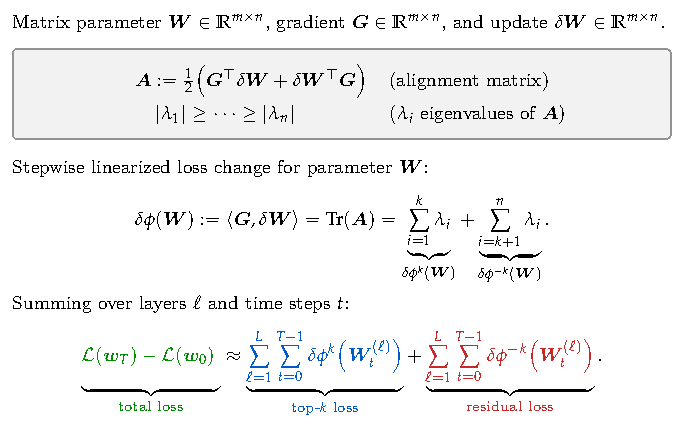
\includegraphics[width=\linewidth, height=13cm, keepaspectratio]{decomposition_equation.pdf}
        \end{column}
        \begin{column}{0.42\linewidth}\centering
          
\includegraphics[width=\linewidth, height=10cm, keepaspectratio]{decomp.png}\\[0.3em]
          {\large\itshape Cartoon: total loss $=$ (U-shaped, width-stable) top-$k$ $+$ (flat) residual.}
        \end{column}
      \end{columns}

      \vspace{0.4em}

      \begin{center}
        \tealbox{\normalsize \textbf{Conjecture} (qualitative). For some $k$: \textbf{(1)} top-$k$ loss is locally strongly convex at its optimum; \textbf{(2)} \emph{top-$k$ invariance} --- $\phi^k_n \approx \phi^k_\infty$, $\nu^{k*}_n \approx \nu^{k*}_\infty$; \textbf{(3)} \emph{residual flatness} --- $\nu^{k*}_n \approx \nu^*_n$.}
      \end{center}

      \vspace{0.5em}

      % ---- Panel D ----
      \panelhead{Experiments}

      {\Large We measure the decomposition on an actual LLM training run. The same three-way split shown in the cartoon appears directly in the data: top-$k$ curves overlap across widths and share the total's optimum, while residuals are flat in the LR.}

      \begin{center}{\large\itshape Setup: 4-layer LLaMA $\cdot$ WikiText-103 $\cdot$ Adam $\cdot$ warmup--stable--decay LR $\cdot$ widths $128$--$2048$ ($n=2048$ as $\infty$-proxy).}\end{center}

      \begin{center}
        
\includegraphics[width=\linewidth, height=12cm, keepaspectratio]{topk-residual.png}
      \end{center}
      \begin{columns}[T, onlytextwidth]
        \begin{column}{0.33\linewidth}\centering
          \textbf{\normalsize Total $\phi_n$}\\ {\footnotesize U-shaped; optima shift with width.}
        \end{column}
        \begin{column}{0.34\linewidth}\centering
          \textbf{\normalsize Top-$k$ $\phi_n^{k_n}$}\\ {\footnotesize Overlap across widths; \emph{same} optimum as total.}
        \end{column}
        \begin{column}{0.33\linewidth}\centering
          \textbf{\normalsize Residual $\phi_n^{-k_n}$}\\ {\footnotesize Flat in LR; can't move the optimum.}
        \end{column}
      \end{columns}

      \vspace{0.4em}
      \begin{center}
        \tealbox{\normalsize All three conjecture pieces (LSC, invariance, flatness) \textbf{verified} on a real LLM run.}
      \end{center}

      \vspace{0.3em}
      {\large\itshape In the paper: provable fast transfer for RF ridge regression; transfer behavior of Muon \& Dion; a data-centric viewpoint of the top-$k$ loss; a $\mu$P failure case. arXiv:2512.22768.}

      \vspace{0.5em}
      \begin{center}
        \orangebox{\parbox{0.95\linewidth}{\large \centering \textbf{Takeaway.} $\mu$P alone only guarantees HP transfer --- not \emph{useful} transfer. What makes tuning a small proxy worthwhile is a \emph{low-rank structure in training}: a small, width-stable top-$k$ component carries the HP signal, while the rest is flat.}}
      \end{center}

    \end{column}
  \end{columns}

\end{frame}
\end{document}
